\documentclass[a4paper]{article}

\usepackage[english]{babel}
\usepackage[utf8]{inputenc}
\usepackage{amsmath}
\usepackage{graphicx}
\usepackage[colorinlistoftodos]{todonotes}
\usepackage[left=2cm, right=2cm, top=2cm]{geometry} 
\usepackage{float}
\title{Homework 2}

%\author{Your names and group number}

\date{\today}

\begin{document}
\maketitle



\begin{figure}[H]
\centering
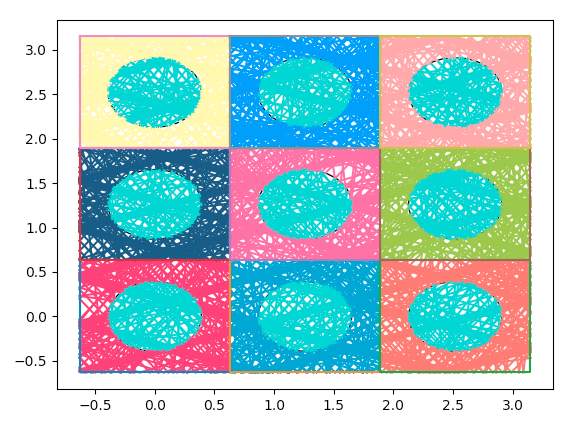
\includegraphics[width=0.8\textwidth]{raysPic}
  \caption{\label{fig:fig1}} Here is a picture of my pincell 3x3 with a lot of rays in it.
\end{figure}







%\begin{thebibliography}{9}
%\bibitem{nano3}
%  K. Grove-Rasmussen og Jesper Nygård,
%  \emph{Kvantefænomener i Nanosystemer}.
%  Niels Bohr Institute \& Nano-Science Center, Københavns Universitet
%
%\end{thebibliography}


\end{document}
